% -- Slide ---------------------------------------------------------------------
\begin{frame}
\frametitle{\bf Outline}

  
\includegraphics[height=0.5in]{images/tachyon-icon.png}
  \begin{minipage}[b]{3.5in}
    \begin{center}
      {\em A hypothetical particle that travels faster than light.} \\
      -- Oxford Dictionary
    \end{center}
  \end{minipage}

  \bigskip

  \begin{itemize}

  \item {\bf System overview} -- {\em Marc Feeley}
    \smallskip

  \item {\bf IR and optimization} -- {\em Maxime Chevalier-Boisvert}
    \smallskip

  \item {\bf Self hosting and back-end} -- {\em Erick Lavoie}
    \smallskip

  \item {\bf Profiling and conclusion} -- {\em Bruno Dufour}
    \smallskip

  \end{itemize}
\end{frame}
% ------------------------------------------------------------------------------

% -- Slide ---------------------------------------------------------------------
\begin{frame}
\frametitle{\bf Goals}

  \begin{itemize}

  \item Tachyon JS project started March 2010
    \smallskip

  \item JS is a key language with a bright future
    \smallskip

  \item 2010 JS VMs performance... {\bf We can do better!}
    \smallskip

    \bigskip

  \item Goal \#1: compiler for research on dynamic languages
    \begin{itemize}
    \item optimistic optimizations
    \item object representation / garbage collection
    \item profiling real-world applications
    \item language extensions: exact arithmetic, continuations, tail calls, exceptions, concurrency, distributed computing, Harmony,~...
    \end{itemize}
    \smallskip

  \item Goal \#2: production-quality high-performance open-source
    JS compiler for client-side and server-side scripting

  \end{itemize}

\end{frame}
% ------------------------------------------------------------------------------

% -- Slide ---------------------------------------------------------------------
\begin{frame}
\frametitle{\bf Current State}

  \begin{itemize}

  \item Compiler is written in a subset of JS (roughly 40 KLOC)
    \begin{itemize}
    \item parsing
    \item analysis/optimization of intermediate representation
    \item in-memory assembly and linking
    \end{itemize}
    \smallskip

  \item Few extensions to the host VM (readFile, malloc, etc.)
    \smallskip

  \item Implements ES5 spec except:
    \begin{itemize}
    \item floating point (only fixnums are supported)
    \item regular expressions
    \item setters and getters
    \item {\tt eval} and most metaprogramming features
    \item no GC!
    \end{itemize}
    \smallskip

  \item Back-end supports {\bf x86} and {\bf x86\_64}
    \smallskip

  \item Tachyon self-bootstrap achieved March 2011
    \smallskip

  \end{itemize}
\end{frame}
% ------------------------------------------------------------------------------

% -- Slide ---------------------------------------------------------------------
\begin{frame}
\frametitle{\bf Parser}

  \begin{itemize}

  \item Based on WebKit's yacc grammar
    \begin{itemize}
    \item {\tt Grammar.y} converted to LALR-SCM parser generator spec
    \item LALR-SCM tables pretty-printed as JS arrays (6 KLOC)
    \item hand written LALR driver (.3 KLOC) and scanner (1 KLOC)
    \end{itemize}
    \smallskip

  \item Parses 100 KLOC per second
    \smallskip

  \item AST keeps track of source location

  \end{itemize}

  \begin{center}
    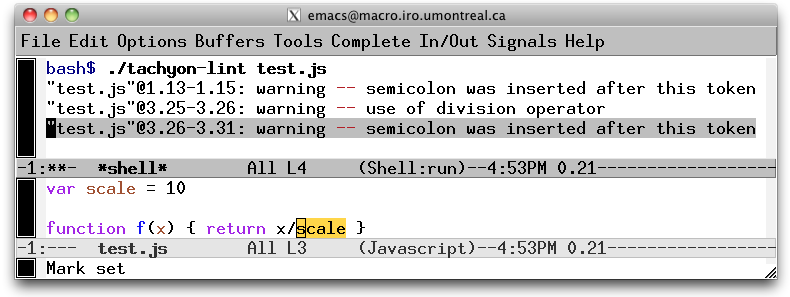
\includegraphics[height=1.5in]{images/tachyon-lint.png}
  \end{center}

\end{frame}
% ------------------------------------------------------------------------------

% -- Slide ---------------------------------------------------------------------
\begin{frame}[fragile]
\frametitle{\bf Parser Derivatives for Debugging}

  \begin{itemize}

  \item {\bf JS pretty-printer} -- dump or pretty print AST
    \smallskip

  \item {\bf js2scm} -- compile JS to Scheme
    \smallskip

  \item {\bf js2js} -- instrument JS code with function entry/exit tracing
    \smallskip

\begin{block}<+->{Execution trace for Tachyon}
\begin{lstlisting}[language=]
bash$ ./js2js -debug tachyon.js > tachyon-debug.js
bash$ d8 tachyon-debug.js
|  (( "utility/iterators.js"@13.1-17.2: Iterator
|  |  (( "utility/debug.js"@73.1-77.2: assertNew
|  |  |  (( "utility/debug.js"@62.1-68.2: isGlobal
|  |  |  |  (( "utility/debug.js"@65.19-65.47: isGlobal
|  |  |  |  )) "utility/debug.js"@65.33-65.45: isGlobal
|  |  |  )) "utility/debug.js"@67.5-67.27: isGlobal
|  |  )) "utility/debug.js"@73.1-77.2: assertNew
|  )) "utility/iterators.js"@16.5-16.17: Iterator
|  (( "utility/iterators.js"@13.1-17.2: Iterator
|  |  (( "utility/debug.js"@73.1-77.2: assertNew
...
\end{lstlisting}
\end{block}

  \end{itemize}

\end{frame}
% ------------------------------------------------------------------------------
